\documentclass[aspectratio=169,xcolor=table]{beamer}
\usetheme[style=classic]{mhar-vell}
%\usepackage{helvet}
%*--------------------------------------------------
\usepackage{bibunits}  
%\setbeamertemplate{bibliography item}{[\theenumiv]}
\setbeamertemplate{bibliography item}{\insertbiblabel}
\defaultbibliography{bibliography}
%\defaultbibliographystyle{IEEEtran}
%\defaultbibliographystyle{amsalpha}
\defaultbibliographystyle{abntex2-alf}
%\bibliography{bibliography}
%\usepackage[backend=biber,style=alphabetic,citestyle=authoryear]{biblatex}
% \addbibresource{bibliography.bib}
%\usepackage{natbib}
\usepackage{bibentry}
%*--------------------------------------------------
\usepackage{epigraph}
\usepackage{graphicx}
\usepackage{multirow}
%\usepackage{enumitem}
\usepackage{array}
%\usepackage{multimedia}
\usepackage{media9}
%\usepackage{pdfpc-movie}
\usepackage{tikz}
\usepackage{circledsteps}
\usepackage{listings}
\usepackage{setspace}
\usepackage[normalem]{ulem}
%\usepackage{Sweave}
%\usepackage{xkeyval}
%\usepackage{palatino}
%\usepackage{pgfpages}
%*--------------------------------------------------
\usepackage[timeinterval=1]{tdclock}
%\usepackage[font=Times,timeinterval=1, timeduration=200,resetatpages=all]{tdclock}
%\usepackage[font=Times,timeinterval=10, timeduration=2.0, timedeath=0, fillcolorwarningsecond=white!60!yellow,timewarningfirst=50,timewarningsecond=80,resetatpages=2]{tdclock}
%*--------------------------------------------------
\usepackage{url}
\usepackage{tabularx,booktabs}
\usepackage{threeparttable}
\usepackage[absolute, overlay]{textpos}
%*--------------------------------------------------
\usepackage{framed, color}
\usepackage[tikz]{bclogo}
\usepackage{spot}
\setspotlightcolor{red!50}
% %\setspotlightstyle{star, fill=red!50}
% %\setspotlightstyle{star points=7}
\usepackage{color,soul}
%\usepackage{xcolor}
\usepackage{tcolorbox}
\usepackage{xcolor}
%*--------------------------------------------------
\usepackage{amsmath}
\usepackage{xfrac}
\usepackage{units}
\usepackage{ulem}
%*-------------------------------------------------------------------------------
%\newcolumntype{C}[1]{>{\centering\arraybackslash}m{#1}}
\newcolumntype{L}[1]{>{\raggedright\let\newline\\\arraybackslash\hspace{0pt}}m{#1}}
\newcolumntype{C}[1]{>{\centering\let\newline\\\arraybackslash\hspace{0pt}}m{#1}}
\newcolumntype{R}[1]{>{\raggedleft\let\newline\\\arraybackslash\hspace{0pt}}m{#1}}
%*-------------------------------------------------------------------------------
%\pgfpagesuselayout{2 on 1}[a4paper,border shrink=5mm]
%\setbeamertemplate{note page}[plain]
%\setbeameroption{show notes on second screen=bottom}
%*-------------------------------------------------------------------------------
\setbeameroption{hide notes}
%\setbeameroption{show only notes}
%\setbeameroption{show notes on second screen=right}
\setbeamertemplate{note page}{\pagecolor{yellow!5}\insertnote}
%*-------------------------------------------------------------------------------
\title              {The Stanford Cart}
\subtitle           {The Stanford Cart and The CMU Rover}
\author             {Juliana Maria S. de Santana}
\email              {juliana.maria@fbter.org.br}
\advisor            {Orientador: Marco A. dos Reis}
\institute          {Robótica e Sistemas Autônomos, Senai Cimatec}
\date               {Outubro de 2021}
% \ulogo        		{Template/logosenaicimatecnegativo}
% \ulogof             {Template/logosenaicimatec2020}
% \ulogoo        		{Template/rosa-logo}
% \ulistelement    	{Template/bullet-white}

%*-------------------------------------------------------------------------------
\graphicspath{{Media/pictures/}}
%*-------------------------------------------------------------------------------
\totalNoSlidesDisabled % To turn off the total number of slides in the footer. Comment this if you want the total number of slides in the footer
%*-------------------------------------------------------------------------------
\begin{document}
%*----------- COVER -------------------------------------------------------------
 \begin{frame}[t,plain]
%*----------- sound--------------------------------
    \includemedia[
        %width=1ex,
        %height=1ex,
        %activate=pageopen, 
        activate=onclick,
        deactivate=onclick,
        %passcontext,
        transparent,
        addresource=./Media/sounds/hip-hop.mp3,
        flashvars={
                    source=./Media/sounds/hip-hop.mp3
                    %&autoPlay=true
                    &autoRewind=true
                    &Play=2s
                    &repeat=always
                    %&Loop=true
        }
    ]
    {}{VPlayer.swf}
%*----------- start-page--------------------------
    \titlepage
%*----------- notes-------------------------------
    \note[item]{Notes can help you to remember important information. Turn on the notes option.}
    \note[item]{Notes can help you to remember important information. Turn on the notes option.}
\end{frame}
%-
%*----------- SECTIONS ----------------------------------------------------------
%\input{Sections/01-introduction}
%\input{Sections/02-review}
%\input{Sections/03-method}
%\input{Sections/04-results}
%\input{Sections/05-references}
%-
%----------FOLLOW-UP SECTIONS ---------------------------------------------------
% %*----------- SLIDE -------------------------------------------------------------

%*----------- SLIDE -------------------------------------------------------------
\begin{frame}[t]{Instruções instalação CoppeliaSim}
Realize o download do software através do link abaixo, de acordo com o seu sistema operacional

\vspace*{0.3cm}
\href{https://www.coppeliarobotics.com/downloads}{Link: CoppeliaSim download}
\vspace*{0.5cm}
\begin{itemize}
    \item Selecione a versão educacional (CoppeliaSim Edu)
    \item Siga as instruções da janela de instalação
\end{itemize}
%*----------- notes
    \note[item]{Notes can help you to remember important information. Turn on the notes option.}
\end{frame}
%-

{
\setbeamertemplate{background}
{\includegraphics[width =\the\paperwidth]{abb-lab.png}}
%*----------- SLIDE -------------------------------------------------------------
\begin{frame}[t]{} 
    % \transdissolve[duration=0.5]

    \vspace*{0.5cm}
    \begin{flushleft}
        \color{black}\Huge{Robôs Industriais}
    \end{flushleft}
    
    \vspace*{-0.5cm}
    \raggedright\color{black}\rule{5.8cm}{0.03cm}

    \vspace*{-0.3cm}
    \begin{flushleft}
        % \color{highlightcolor}\scriptsize{Aspectos da indústria}
    \end{flushleft}

%*----------- notes
    \note[item]{Notes can help you to remember important information. Turn on the notes option.}
\end{frame}
}
%-
%*----------- SLIDE -------------------------------------------------------------
\begin{frame}[c]{} 
    % \transdissolve[duration=0.5]
   
    \begin{center}
        \Wider{%
        \begin{shaded}
        \begin{center}
            \vspace*{0.3cm}
            \resizebox{!}{0.6cm}{%
                Cinemática
            }%
        \end{center}
        \end{shaded}
        }%
    \end{center}
       
%*----------- notes
    \note[item]{Notes can help you to remember important information. Turn on the notes option.}
\end{frame}
%*----------- SLIDE -------------------------------------------------------------
\begin{frame}[c]{Cinemática direta vs inversa}
    \begin{columns}
        \column{.01\textwidth}
        \column{.50\textwidth}
        Cinemática Direta
        \begin{itemize}
            \item Encontrar a posição e orientação
            \item São dados os ângulos de junta
        \end{itemize}
        Cinemática Inversa
        \begin{itemize}
            \item Encontrar os ângulos de junta
            \item São dados a posição e orientação
        \end{itemize}
        \column{.5\textwidth}
            \centering
            \includegraphics[width=\textwidth, clip, trim = 0 0 0 0]{ik-matlab.jpg}
    \end{columns}
%*----------- notes
    \note[item]{Notes can help you to remember important information. Turn on the notes option.}
\end{frame}
%-
%*----------- SLIDE -------------------------------------------------------------
\begin{frame}[c]{Qual a importância da cinemática inversa ?}
    \begin{columns}
        \column{.01\textwidth}
        \column{.48\textwidth}
        \begin{itemize}
            \item Permite o robô atingir as posições e orientações desejadas
            \item Encontra os valores exatos de ângulos para cada junta
        \end{itemize}
        \column{.55\textwidth}
            \centering
            \begin{figure}
                \roundpic[xshift=0cm,yshift=0cm]{6cm}{6cm}{ur5.jpg}
            \end{figure}
    \end{columns}
%*----------- notes
    \note[item]{Notes can help you to remember important information. Turn on the notes option.}
\end{frame}
%-
%*----------- SLIDE -------------------------------------------------------------
\begin{frame}[c]{Metodologia para solucionar IK}
    %\transboxout[duration=0.5]
    \centering
    \includegraphics[width=
    \textwidth, clip, trim = 0 0 0 0]{esquematico.png}
%*----------- notes
    \note[item]{Notes can help you to remember important information. Turn on the notes option.}
\end{frame}
%-
%*----------- SLIDE -------------------------------------------------------------
\begin{frame}[c]{} 
    % \transdissolve[duration=0.5]
   
    \begin{center}
        \Wider{%
        \begin{shaded}
        \begin{center}
            \vspace*{0.3cm}
            \resizebox{!}{0.7cm}{%
                Descrições mecânicas
            }%
        \end{center}
        \end{shaded}
        }%
    \end{center}
       
%*----------- notes
    \note[item]{Notes can help you to remember important information. Turn on the notes option.}
\end{frame}
%*----------- SLIDE -------------------------------------------------------------
\begin{frame}[c]{Anatomia dos manipuladores}
    Principais partes de um manipulador
    \vspace*{0.3cm}
    \begin{columns}
        \column{.01\textwidth}
        \column{.3\textwidth}
        \begin{itemize}
            \item Efetuador
            \item Base 
            \item Actuadores
            \item Sensores  
        \end{itemize}
            \column{.69\textwidth}
            \centering
            \includegraphics[width=0.8\textwidth, clip, trim = 0 0 0 0]{manipulator-caracteristics.png}
    \end{columns}
%*----------- notes
    \note[item]{Notes can help you to remember important information. Turn on the notes option.}
\end{frame}
%-
%*----------- SLIDE -------------------------------------------------------------
\begin{frame}[c]{Anatomia dos manipuladores}
    \begin{columns}
        \column{.01\textwidth}
        \column{.35\textwidth}
        \begin{itemize}
            \item Elos: São membros rígidos entre as juntas 
            \item Juntas: é uma conexão entre dois ou mais
            links, o que permite algum movimento, ou movimento
            potencial, entre os links conectados     
        \end{itemize}
            \column{.5\textwidth}
            \centering
            \includegraphics[width=\textwidth, clip, trim = 0 0 0 0]{manipulator-caracteristics.png}
    \end{columns}
%*----------- notes
    \note[item]{Notes can help you to remember important information. Turn on the notes option.}
\end{frame}
%-
%*----------- SLIDE ------------------------------------------------------------
\begin{frame}
    %\transdissolve[duration=0.5]
    %\hspace*{-1cm}
    \begin{columns}
        %\column{.01\textwidth}
        \column{0.50\textwidth}
        ~\hfill
            \begin{beamercolorbox}[sep=8em, colsep*=18pt, wd=\textwidth,ht=\paperheight]{title page header}
                \begin{center}
                    \textbf{\huge{GRAUS DE}}\par
                    \vspace*{0.3cm}
                    \textbf{\huge{LIBERDADE}}\par
                    \vspace*{0.3cm}
                    é definido como a maneira pela qual um robô ou máquina pode se mover.
                \end{center}
            \end{beamercolorbox}%         
        \column{.05\textwidth} 
        \column{.65\textwidth}
        \begin{center}
            \includegraphics[width=.8\textwidth]{gdl.png}
        \end{center}
            
    \end{columns}
  
%*----------- notes
    \note[item]{Notes can help you to remember important information. Turn on the notes option.}
 \end{frame}
%-
%*----------- SLIDE -------------------------------------------------------------
\begin{frame}[c]{Graus de liberdade}
    Um objeto no espaço possui seis graus de liberdade
    \begin{columns}
        \column{.01\textwidth}
        \column{.35\textwidth}
        \begin{itemize}
            \item Movimento de translação ao longo dos eixos X, Y e Z (3 D.O.F.)
            \item Movimento giratório sobre os eixos X, Y e Z (3 D.O.F)    
        \end{itemize}
            \column{.5\textwidth}
            \centering
            \includegraphics[width=\textwidth, clip, trim = 0 0 0 0]{dof.png}
    \end{columns}
%*----------- notes
    \note[item]{Notes can help you to remember important information. Turn on the notes option.}
\end{frame}
%-
%*----------- SLIDE -------------------------------------------------------------
\begin{frame}[t]{Graus de liberdade}
    \begin{columns}
        \column{.01\textwidth}
        \column{.35\textwidth}
O corpo rígido possui 6 GDL, porém possuem algumas restrições devido as suas ligações

\vspace*{0.3cm}

Portanto apresentam um número menor de graus de liberdade
            \column{.5\textwidth}
            \centering
            \includegraphics[width=0.8\textwidth, clip, trim = 0 0 0 0]{braco-dof.png}
    \end{columns}
%*----------- notes
    \note[item]{Notes can help you to remember important information. Turn on the notes option.}
\end{frame}
%-
%*----------- SLIDE -------------------------------------------------------------
\begin{frame}[c]{Tipos de juntas}
    %\transboxout[duration=0.5]
    \centering
    \includegraphics[width=0.8\textwidth, clip, trim = 0 0 0 0]{tipos-juntas.png}
%*----------- notes
    \note[item]{Notes can help you to remember important information. Turn on the notes option.}
\end{frame}
%-
%*----------- SLIDE -------------------------------------------------------------
\begin{frame}[t]{URDF}
    \framesubtitle{aplicação}
    \begin{columns}
        \column{.01\textwidth}
        \column{.55\textwidth}
            \begin{itemize}
                \item É uma especificação XML para descrever robôs 
                \item A descrição consiste de elos e juntas   
                \item Utiliza arquivos gerados em CAD
            \end{itemize} 
            \vspace*{0.3cm}
            \href{https://mhar-vell.github.io/rasc/2021-07-21-aperea-simulacao/}{Exemplo: projeto APEREA}
        \column{.5\textwidth}
            \centering
            \includegraphics[width=\textwidth, clip, trim = 0 0 0 0]{urdf.png}
    \end{columns}
%*----------- notes
    \note[item]{Notes can help you to remember important information. Turn on the notes option.}
\end{frame}
%-
%*----------- SLIDE -------------------------------------------------------------
\begin{frame}[c]{} 
    % \transdissolve[duration=0.5]
   
    \begin{center}
        \Wider{%
        \begin{shaded}
        \begin{center}
            \vspace*{0.3cm}
            \resizebox{!}{0.6cm}{%
                Descrições espaciais 
                e transformações
            }%
        \end{center}
        \end{shaded}
        }%
    \end{center}
       
%*----------- notes
    \note[item]{Notes can help you to remember important information. Turn on the notes option.}
\end{frame}
%*----------- SLIDE -------------------------------------------------------------
\begin{frame}[t]{Descrição de uma posição}
    Descrever a posição de um ponto no espaço
    \vspace*{0.3cm}
    \begin{columns}
        \column{.01\textwidth}
        \column{.3\textwidth}
        \begin{itemize}
            \item \textbf{Vetor de posição} 3x1
        \end{itemize}
        \column{.69\textwidth}
            \centering
            \includegraphics[width=\textwidth, clip, trim = 0 0 0 0]{posicao.png}
    \end{columns}
%*----------- notes
    \note[item]{Notes can help you to remember important information. Turn on the notes option.}
\end{frame}
%-
%*----------- SLIDE -------------------------------------------------------------
\begin{frame}[c]{Descrição de uma orientação}
    Indica a localização completa de um ponto
    \begin{columns}
        \column{.01\textwidth}
        \column{.49\textwidth}
        \begin{itemize}
            \item Fixar um sistema de coordenadas
            \item Descrever com relação à um sistema de referência
            \item Matriz rotacional 3x3
        \end{itemize}
        \column{.5\textwidth}
            \centering
            \includegraphics[width=0.6\textwidth, clip, trim = 0 0 0 0]{orientação.png}
    \end{columns}
%*----------- notes
    \note[item]{Notes can help you to remember important information. Turn on the notes option.}
\end{frame}
%-
%*----------- SLIDE -------------------------------------------------------------
\begin{frame}[c]{Descrição de um sistema de referência}
    \begin{columns}
        \column{.01\textwidth}
        \column{.49\textwidth}
        \begin{itemize}
            \item Atribuição de nomes e localização
            \item Considera o robô e seu espaço de trabalho
            \item Os movimentos robóticos podem ser descritos em termos desses sistemas
        \end{itemize}
        \column{.55\textwidth}
            \centering
            \includegraphics[width=\textwidth, clip, trim = 0 0 0 0]{sist=referencia2.png}
    \end{columns}
%*----------- notes
    \note[item]{Notes can help you to remember important information. Turn on the notes option.}
\end{frame}
%-
%*----------- SLIDE -------------------------------------------------------------
% \begin{frame}[c]{Descrição de um sistema de referência}
%     \begin{columns}
%         \column{.01\textwidth}
%         \column{.35\textwidth}
%         \includegraphics[width=\textwidth, clip, trim = 0 0 0 0]{referencia.png}
%         \column{.5\textwidth}
%             \centering
%             \includegraphics[width=\textwidth, clip, trim = 0 0 0 0]{referencia2.png}
%     \end{columns}
%*----------- notes
%     \note[item]{Notes can help you to remember important information. Turn on the notes option.}
% \end{frame}
%-
%*----------- SLIDE -------------------------------------------------------------
\begin{frame}[c]{Descrição de um sistema de referência}
    \begin{columns}
        \column{.01\textwidth}
        \column{.49\textwidth}
        \begin{itemize}
            \item O sistema de referência da base (base frame) {B}
            \item O sistema de referência da estação (station frame) {S}
            \item O sistema de referência do punho (wrist frame) {W}
            \item O sistema de referência da ferramenta (tool frame) {T}
            \item O sistema de referência meta (goal frame) {G}
        \end{itemize}
        \column{.55\textwidth}
            \centering
            \includegraphics[width=\textwidth, clip, trim = 0 0 0 0]{sist=referencia2.png}
    \end{columns}
%*----------- notes
    \note[item]{Notes can help you to remember important information. Turn on the notes option.}
\end{frame}
%-
%*----------- SLIDE -------------------------------------------------------------
\begin{frame}[c]{Transformação homogênea}
    \begin{columns}
        \column{.01\textwidth}
        \column{.35\textwidth}

        Dispõe a rotação e a translação da transformação geral na forma de uma única matriz
        \column{.64\textwidth}
            \centering
            \includegraphics[width=\textwidth, clip, trim = 0 0 0 0]{trans-homogenea.png}
    \end{columns}
%*----------- notes
    \note[item]{Notes can help you to remember important information. Turn on the notes option.}
\end{frame}
%-
%-
%*----------- SLIDE -------------------------------------------------------------
\begin{frame}[c]{} 
    % \transdissolve[duration=0.5]
   
    \begin{center}
        \Wider{%
        \begin{shaded}
        \begin{center}
            \vspace*{0.3cm}
            \resizebox{!}{0.6cm}{%
                Cinemática
            }%
        \end{center}
        \end{shaded}
        }%
    \end{center}
       
%*----------- notes
    \note[item]{Notes can help you to remember important information. Turn on the notes option.}
\end{frame}
%*----------- SLIDE -------------------------------------------------------------
\begin{frame}[t]{Cinemática direta} 
    % \transdissolve[duration=0.5]
    
    \begin{columns}[c]
        \column{0.01\linewidth}
        \column{0.3\linewidth}
        A cinemática direta, considerando um manipulador, possui como 
        entrada os ângulos das junta e calcula a posição cartesiana e 
        a orientação do end-effector 
        \column{0.69\linewidth}
            \begin{figure}
                \roundpic[xshift=0cm,yshift=0cm]{6cm}{6cm}{manipulador2.jpg}
            \end{figure}
    \end{columns}
%*----------- notes
    \note[item]{Notes can help you to remember important information. Turn on the notes option.}
\end{frame}
%-
%*----------- SLIDE -------------------------------------------------------------
\begin{frame}[t]{Cinemática direta} 
    % \transdissolve[duration=0.5]
    \begin{columns}[c]
        \column{0.01\linewidth}
        \column{0.49\linewidth}
        \begin{figure}
            \roundpic[xshift=0cm,yshift=0cm]{6cm}{6cm}{dobot.jpg}
        \end{figure} 
        \column{0.5\linewidth}
        As equações da cinemática direta serão definidas através de uma abordagem sistemática e geral baseada na álgebra linear 
    \end{columns}
%*----------- notes
    \note[item]{Notes can help you to remember important information. Turn on the notes option.}
\end{frame}
%-
%*----------- SLIDE -------------------------------------------------------------
\begin{frame}[c]{Notação de Denavit-Hartenberg }
    \begin{columns}
        \column{.01\textwidth}
        \column{.3\textwidth}
        Os parâmetros de Denavit-Hartenberg são quatro 
        parâmetros associados a uma convenção particular, a qual relaciona frames de referências aos links de uma cadeia cinemática 
        \column{.69\textwidth}
            \centering
            \includegraphics[width=0.6\textwidth, clip, trim = 0 0 0 0]{para.png}
    \end{columns}
%*----------- notes
    \note[item]{Notes can help you to remember important information. Turn on the notes option.}
\end{frame}
%-
%*----------- SLIDE -------------------------------------------------------------
\begin{frame}[t]{Notação de Denavit-Hartenberg} 
    % \transdissolve[duration=0.5]
    
    \begin{columns}[c]
        \column{0.01\linewidth}
        \column{0.3\linewidth}
        Jacques Denavit (1930-2012)
        \begin{itemize}
            \item Doutor em Engenharia mecânica
            \item Em 1958, juntou-se ao Departamento de Engenharia
            mecânica e ciência astronautica
            \item Interessado em dinâmica e cinemática
              \end{itemize}
        \column{0.69\linewidth}
            \begin{figure}
                \roundpic[xshift=0cm,yshift=0cm]{6cm}{6cm}{jacques-fenavit.png}
            \end{figure}
    \end{columns}
%*----------- notes
    \note[item]{Notes can help you to remember important information. Turn on the notes option.}
\end{frame}
%-
%-
%*----------- SLIDE -------------------------------------------------------------
\begin{frame}[t]{Notação de Denavit-Hartenberg} 
    % \transdissolve[duration=0.5]
    
    \begin{columns}[c]
        \column{0.01\linewidth}
        \column{0.3\linewidth}
        Richard Hartenberg (1907-1997)
        \begin{itemize}
            \item Foi professor de engenharia mecânica por 56 anos

            \item Contribui extensivamente na área da engenharia mecânica
              \end{itemize}
        \column{0.69\linewidth}
            \begin{figure}
                \roundpic[xshift=0cm,yshift=0cm]{6cm}{6cm}{richard-hartenberg.png}
            \end{figure}
    \end{columns}
%*----------- notes
    \note[item]{Notes can help you to remember important information. Turn on the notes option.}
\end{frame}
%-
%*----------- SLIDE -------------------------------------------------------------
\begin{frame}[c]{Notação de Denavit-Hartenberg}
    \begin{columns}
        \column{.01\textwidth}
        \column{.48\textwidth}
        \begin{itemize}
            \item É uma convenção comumente usada para selecionar frames de
            referência em aplicações de robótica
            \item Frames de coordenadas são anexados às juntas de forma que, uma transformação é associada a uma junta e a segunda é associada ao link
        \end{itemize}
        \column{.55\textwidth}
            \centering
            \includegraphics[width=\textwidth, clip, trim = 0 0 0 0]{DHParameter.png}
    \end{columns}
%*----------- notes
    \note[item]{Notes can help you to remember important information. Turn on the notes option.}
\end{frame}
%-
%*----------- SLIDE -------------------------------------------------------------
\begin{frame}[c]{Matriz de Denavit-Hartenberg}
    \begin{columns}
        \column{.01\textwidth}
        \column{.48\textwidth}
        \begin{itemize}
            \item Forma geral da transformação que relaciona os sistemas de referência fixados a elos vizinhos
            \item É feita a concatenação das transformações individuais para
            encontrar a posição e a orientação do elo n com relação ao elo 0
        \end{itemize}
        \column{.55\textwidth}
            \centering
            \includegraphics[width=\textwidth, clip, trim = 0 0 0 0]{DH-matrix.png}
    \end{columns}
%*----------- notes
    \note[item]{Notes can help you to remember important information. Turn on the notes option.}
\end{frame}
%-
%*----------- SLIDE -------------------------------------------------------------
\begin{frame}[t]{Cinemática inversa} 
    % \transdissolve[duration=0.5]
    
    \begin{columns}[c]
        \column{0.01\linewidth}
        \column{0.3\linewidth}
            A cinemática inversa, considerando um manipulador,
            tem como entrada a posição e orientação cartesiana do end-effector
        \column{0.69\linewidth}
            \begin{figure}
                \roundpic[xshift=0cm,yshift=0cm]{6cm}{6cm}{ergo.jpg}
            \end{figure}
    \end{columns}
%*----------- notes
    \note[item]{Notes can help you to remember important information. Turn on the notes option.}
\end{frame}
%-
%*----------- SLIDE -------------------------------------------------------------
\begin{frame}[c]{Cinemática inversa}
    \begin{columns}
        \column{.01\textwidth}
        \column{.48\textwidth}
        Pode ter
        \begin{itemize} 
            \item Múltiplas soluções
            \item Nenhuma solução
        \end{itemize}
        \singlespacing
            Possui vários métodos para resolução
        \column{.55\textwidth}
            \centering
            \includegraphics[width=\textwidth, clip, trim = 0 0 0 0]{sist-referencia-example.png}
    \end{columns}
%*----------- notes
    \note[item]{Notes can help you to remember important information. Turn on the notes option.}
\end{frame}
%-
%*----------- SLIDE -------------------------------------------------------------
\begin{frame}[c]{Categorias de soluções}
    \begin{columns}
        \column{.01\textwidth}
        \column{.49\textwidth}
        \includegraphics[width=0.8\textwidth, clip, trim = 0 0 0 0]{Automationoffoundrywithrobot.jpg}
        \column{.5\textwidth}
            % \centering
            Soluções de forma fechada
            \begin{itemize} 
                \item Método Algébrico
                \item Método Geométrico
                \item Solução de Pieper
            \end{itemize}
            \singlespacing
            Soluções em forma aberta
            \begin{itemize}
                \item Métodos Numéricos
                 \end{itemize}
            % \includegraphics[width=0.8\textwidth, clip, trim = 0 0 0 0]{colab-logo.png}
    \end{columns}
%*----------- notes
    \note[item]{Notes can help you to remember important information. Turn on the notes option.}
\end{frame}
%-
%*----------- SLIDE -------------------------------------------------------------
\begin{frame}[c]{Prática 1 - Resolução questão no Google Colab}
    \begin{columns}
        \column{.01\textwidth}
        \column{.50\textwidth}
        Google Colab
        \begin{itemize} 
            \item Colab é um ambiente de desenvolvimento Python executado no 
            navegador usando o Google Cloud
        \end{itemize}
        \singlespacing
        Bibliotecas:
        \begin{itemize}
            \item SymPy: é uma biblioteca Python para matemática simbólica
            \item Math: é um módulo integrado que fornece uma série de métodos e constantes matemáticas
        \end{itemize}
        \column{.5\textwidth}
            \centering
            \includegraphics[width=0.8\textwidth, clip, trim = 0 0 0 0]{colab-logo.png}
    \end{columns}
%*----------- notes
    \note[item]{Notes can help you to remember important information. Turn on the notes option.}
\end{frame}
%-
%*----------- SLIDE -------------------------------------------------------------
\begin{frame}[c]{Solucionadores}
    \begin{columns}
        \column{.01\textwidth}
        \column{.50\textwidth}
        \includegraphics[width=0.8\textwidth, clip, trim = 0 0 0 0]{FactoryAutomationRoboticsPalettizingBread.jpg}
        \column{.5\textwidth}
        \begin{itemize}
            \item Existem vários métodos de modelagem e solução de problemas de cinemática inversa 
            \singlespacing
            \item Todo método para solucionar a cinemática inversa tem alguns pontos positivos e negativos
        \end{itemize}
            % \includegraphics[width=0.8\textwidth, clip, trim = 0 0 0 0]{}
    \end{columns}
%*----------- notes
    \note[item]{Notes can help you to remember important information. Turn on the notes option.}
\end{frame}
%-
%*----------- SLIDE -------------------------------------------------------------
\begin{frame}[c]{MoveIt}
    \begin{columns}
        \column{.01\textwidth}
        \column{.48\textwidth}
        \begin{itemize}
            \item É um pacote do ROS
            \item É utilizado por diversas empresas
        \end{itemize}
        \singlespacing
        Algumas funcionalidades
        \begin{itemize}
            \item Realiza o cáculo da cinemática inversa
            \item Faz o planejamento de trajetórias
            \item Verifica a presença de obstáculos
        \end{itemize}
        \column{.5\textwidth}
            \centering
            \includegraphics[width=\textwidth, clip, trim = 0 0 0 0]{MOVEIT.png}
    \end{columns}
%*----------- notes
    \note[item]{Notes can help you to remember important information. Turn on the notes option.}
\end{frame}
%-
%*----------- SLIDE -------------------------------------------------------------
\begin{frame}[c]{Prática 2 - Simulação no CoppeliaSim}
    \begin{columns}
        \column{.01\textwidth}
        \column{.50\textwidth}
        V-REP - Virtual Robot Experimentation Platform
        \begin{itemize} 
            \item Simulador de robô de uso geral
        \end{itemize}
        \singlespacing
        Métodos utilizados para resolução
        \begin{itemize}
            \item Método pseudo-inverso 
            \item Método damped least square
        \end{itemize}
        \column{.5\textwidth}
            \centering
            \includegraphics[width=0.8\textwidth, clip, trim = 0 0 0 0]{v-rep.png}
    \end{columns}
%*----------- notes
    \note[item]{Notes can help you to remember important information. Turn on the notes option.}
\end{frame}
%-
  % Figura do que é o projeto / Andamento do projeto
%*----------- SLIDE ------------------------------------------------------------
\begin{frame}
    %\transdissolve[duration=0.5]
    %\hspace*{-1cm}
    \begin{columns}
        %\column{.01\textwidth}
        \column{0.30\textwidth}
        ~\hfill
            \begin{beamercolorbox}[sep=8em, colsep*=18pt, wd=\textwidth,ht=\paperheight]{title page header}
                \begin{center}
                    \textbf{\huge{Introdução}}\par
                    \vspace*{0.3cm}
                    % \textbf{\huge{LIBERDADE}}\par
                    \vspace*{0.3cm}
                    The Stanford Cart and The CMU Rover
                \end{center}
            \end{beamercolorbox}%         
        \column{.05\textwidth} 
        \column{.65\textwidth}
        \begin{center}
            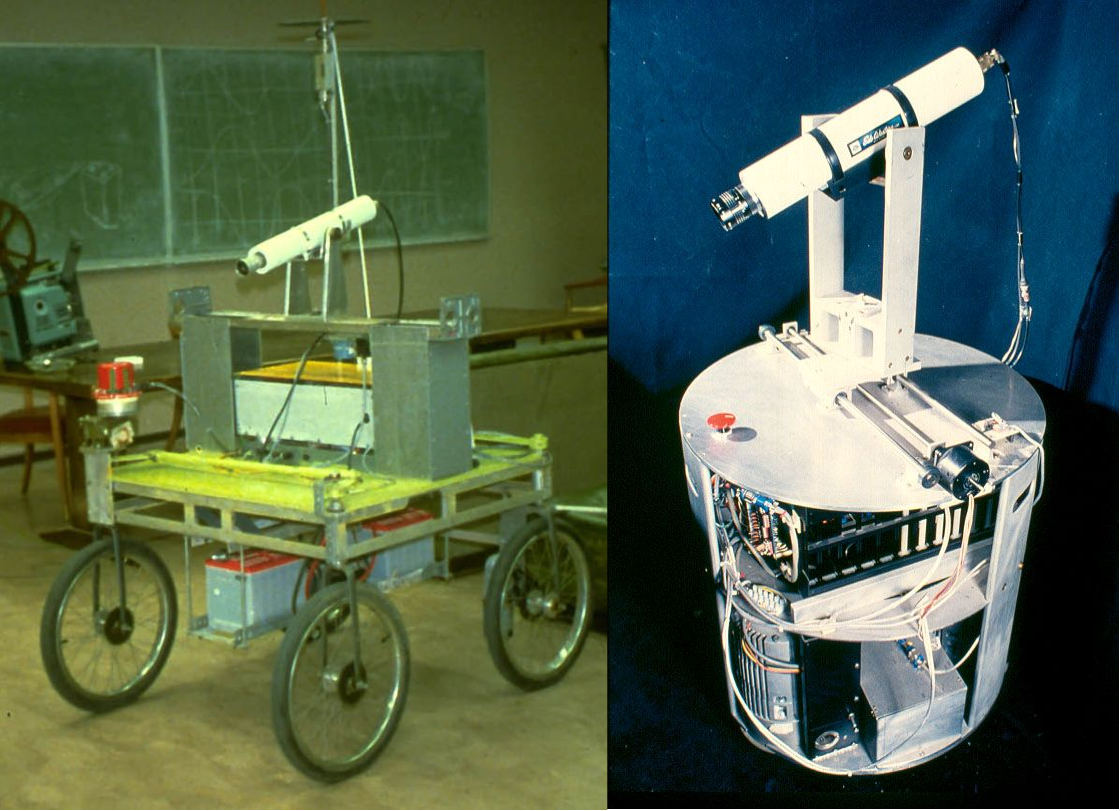
\includegraphics[width=\textwidth]{TheStanfordCart/intro.png}
        \end{center}
            
    \end{columns}
  
%*----------- notes
    \note[item]{Notes can help you to remember important information. Turn on the notes option.}
 \end{frame}
%-
%*----------- SLIDE -------------------------------------------------------------
\begin{frame}[t]{The Stanford Cart}
    \begin{columns}
        \column{.05\textwidth}
        \column{.45\textwidth}
        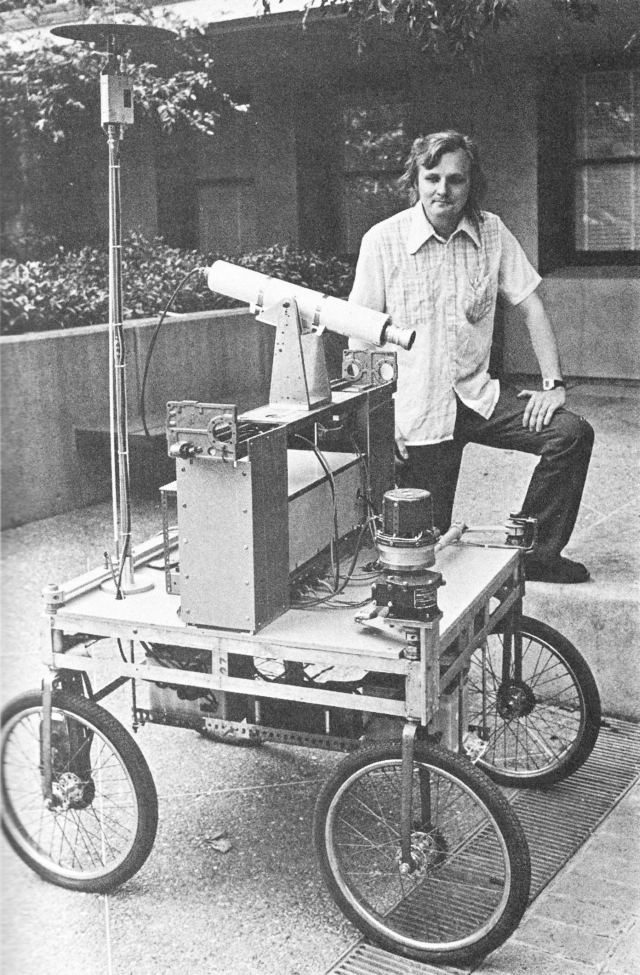
\includegraphics[width=0.6\textwidth, clip, trim = 0 0 0 0]{TheStanfordCart/StanfordCart-Moravec-x640.jpg}
        \column{.5\textwidth}
            % \centering
            Robô móvel equipado com uma câmera de TV
            \begin{itemize} 
                \item Desenvolvido por Hans. P. Moravec
                \item Utiliza visão stereo
                \item Utilizados em pesquisas de navegação visual
            \end{itemize}
            \end{columns}
%*----------- notes
    \note[item]{Notes can help you to remember important information. Turn on the notes option.}
\end{frame}

%*----------- SLIDE -------------------------------------------------------------
\begin{frame}[t]{The Stanford Cart - Rotinas}
    \begin{columns}
        \column{.01\textwidth}
        \column{.49\textwidth}
        O robô obtêm 9 fotos através de sua câmera, e a partir destas é capaz de
        deduzir a transfromada da sua coordenada 3D e a posição 3D dos features das imagens

        \vspace*{0.8cm}
        
\includegraphics[width=\textwidth, clip, trim = 0 0 0 0]{TheStanfordCart/diagram.png}
        \vspace*{0.3cm}
        \column{.5\textwidth}
            % \centering
            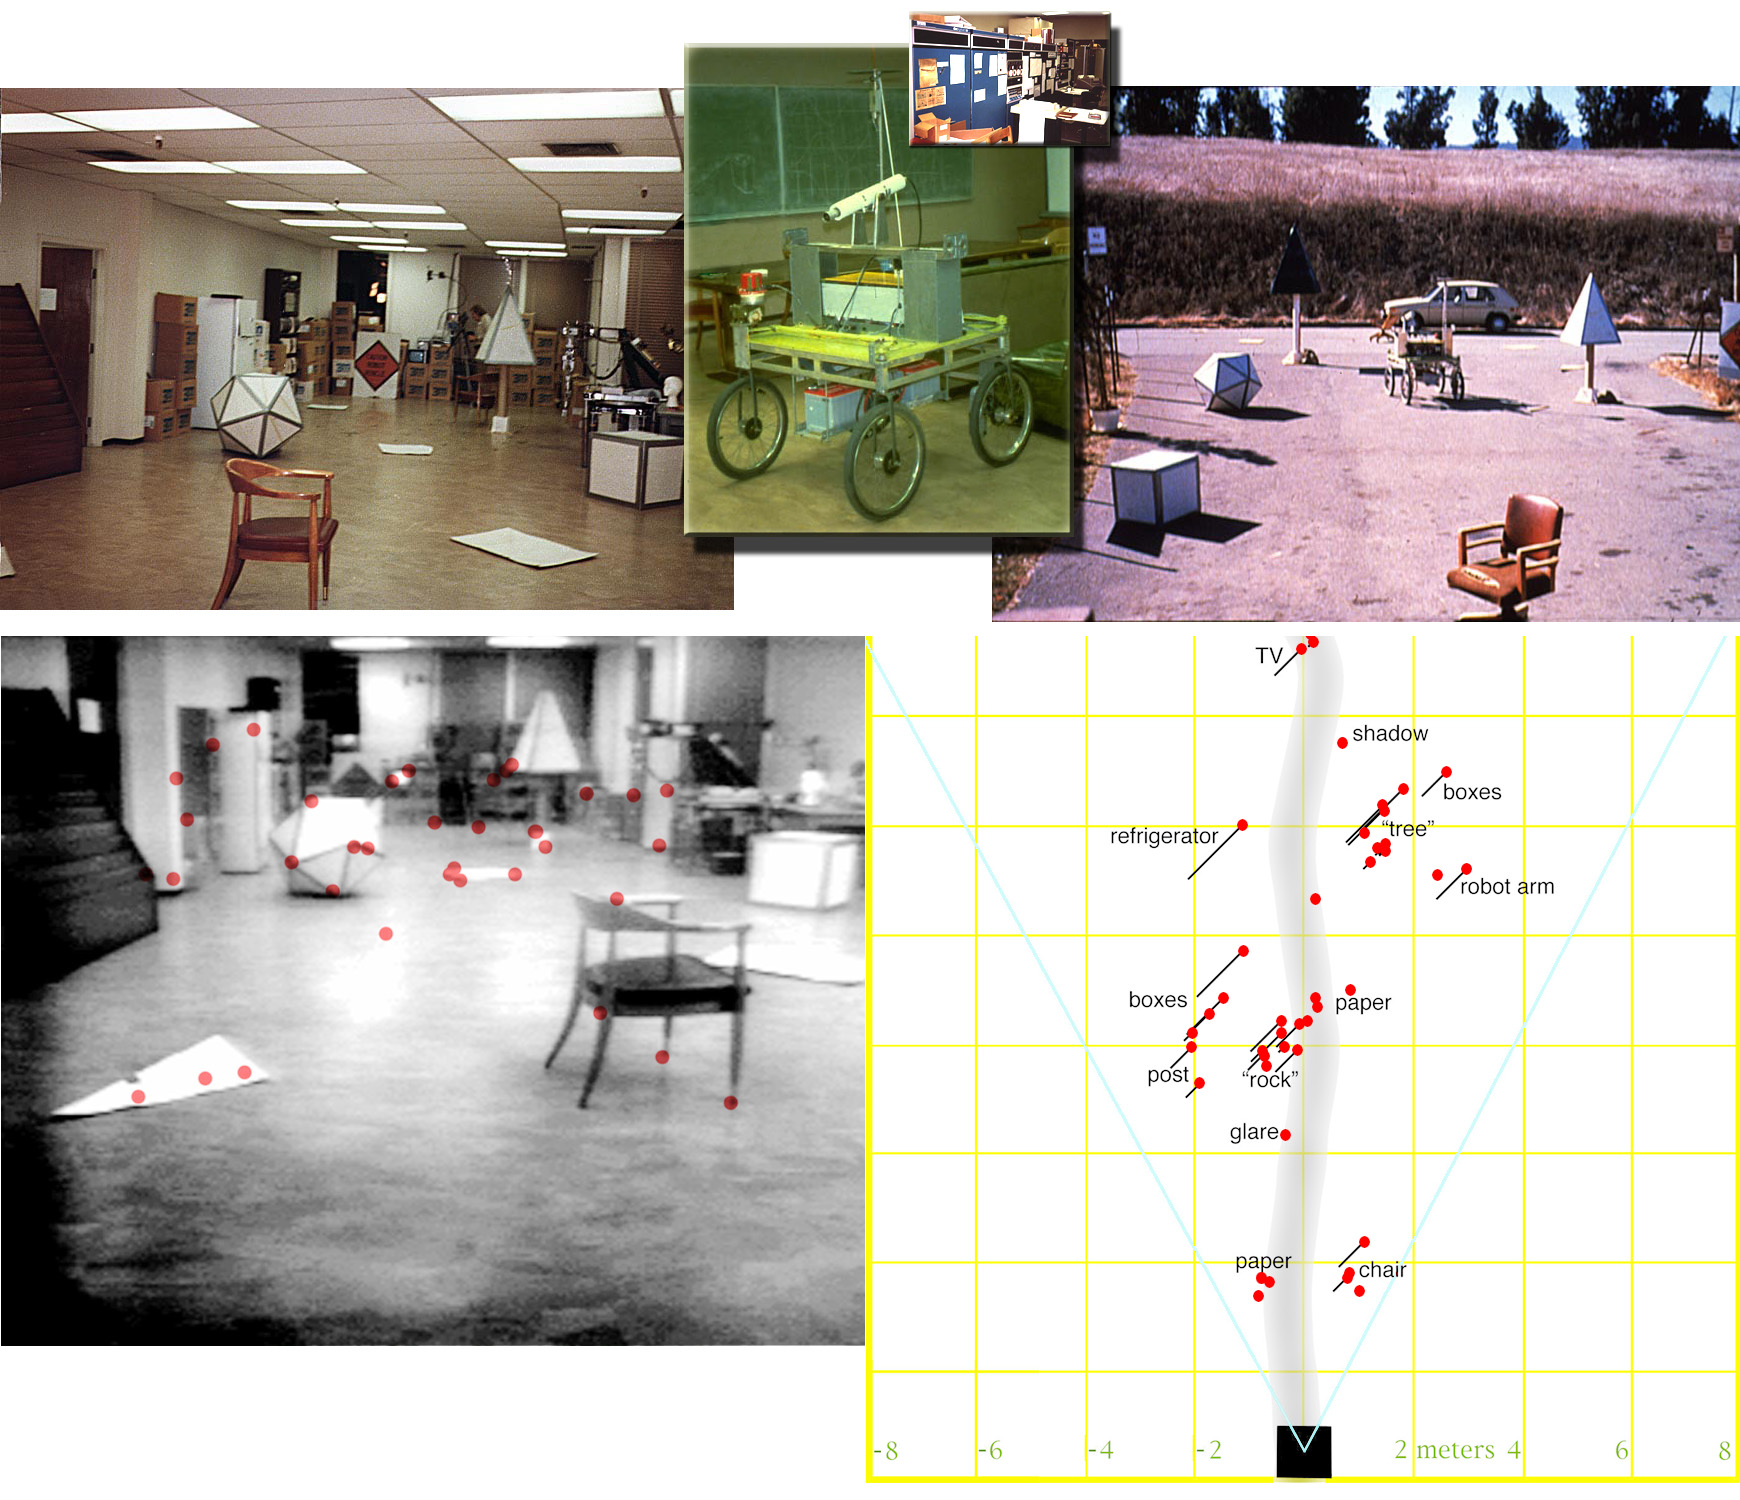
\includegraphics[width=\textwidth, clip, trim = 0 0 0 0]{TheStanfordCart/1979.MRL.image.jpg}
            \end{columns}
%*----------- notes
    \note[item]{Notes can help you to remember important information. Turn on the notes option.}
\end{frame}
%-
%*----------- SLIDE -------------------------------------------------------------
\begin{frame}[c]{Observações dos experimentos}
    \begin{columns}
        \column{.05\textwidth}
        \column{.45\textwidth}
        \begin{itemize} 
            \item Melhores resultados: Ambiente indoor
            \item Tempo de pausa: 10 a 15 minutos
            \item Tempo de execução do percurso: 5 horas
        \end{itemize}
        \column{.5\textwidth}
            \centering
            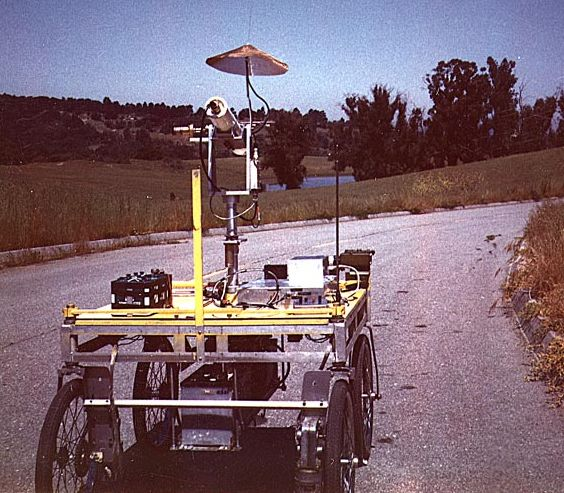
\includegraphics[width=0.8\textwidth, clip, trim = 0 0 0 0]{TheStanfordCart/StanfordCart-005.png}
            \end{columns}
%*----------- notes
    \note[item]{Notes can help you to remember important information. Turn on the notes option.}
\end{frame}

%*----------- SLIDE -------------------------------------------------------------
\begin{frame}[t]{The CMU Rover}
    \begin{columns}
        \column{.05\textwidth}
        \column{.45\textwidth}
        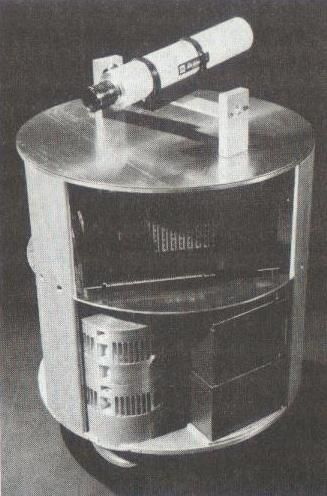
\includegraphics[width=0.6\textwidth, clip, trim = 0 0 0 0]{TheStanfordCart/CMU-Rover-Hollandp2-x640.jpg}
        \column{.5\textwidth}
            % \centering
           Comparação com o Stanford Cart
            \begin{itemize} 
                \item Possui um sistema mais sofisticado
                \item É mais rápido
                \item Possui um sistema mais flexível
            \end{itemize}
            \end{columns}
%*----------- notes
    \note[item]{Notes can help you to remember important information. Turn on the notes option.}
\end{frame}

%*----------- SLIDE -------------------------------------------------------------
\begin{frame}[c]{Características do CMU Rover}
    \begin{columns}
        \column{.05\textwidth}
        \column{.45\textwidth}
        \begin{itemize} 
            \item É cilindrico
            \item Possui 3 GDL nas rodas
            \item Apresenta vários sensores
        \end{itemize}
        \column{.5\textwidth}
            \centering
            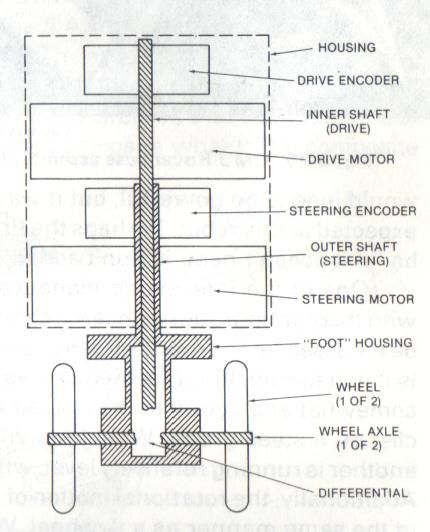
\includegraphics[width=0.75\textwidth, clip, trim = 0 0 0 0]{TheStanfordCart/CMU-Rover-Hollandp3-x640.jpg}
            \end{columns}
%*----------- notes
    \note[item]{Notes can help you to remember important information. Turn on the notes option.}
\end{frame}
%*----------- SLIDE-BACKUP ------------------------------------------------------
% \backupbegin
% %
% \begin{frame}{Backup}
%     Test
% %*----------- notes-------------------------------
% \note{Notes can help you to remember important information. Turn on the notes option.}
% \end{frame}
% %-
% \backupend
% %-
%*----------- QUESTIONS ---------------------------------------------------------
\begin{frame}[c,plain]
    \lastpage{
        \begin{center}   
            {\usebeamerfont{title} Questions?}\\[3ex] 
            %\hspace{1.5cm} 
            juliana.maria@fbter.org.br
        \end{center}
    }
    
%*----------- notes---------------------------------
    \note[item]{Notes can help you to remember important information. Turn on the notes option.}
\end{frame}
%*-------------------------------------------------------------------------------
\end{document}